\documentclass[12pt]{exam}
\usepackage[margin=.75cm,papersize={8.5in,17in}]{geometry}
\usepackage{enumitem}
\usepackage{tikz}
\usepackage{newtxtext,newtxmath}
%\usepackage[document]{ragged2e}
\usepackage[none]{hyphenat}
\usepackage{siunitx}
\usepackage{multicol}
%\usepackage{fancyhdr}

\usetikzlibrary{patterns}

%\renewcommand{\headrulewidth}{0pt}

%\pagestyle{fancy}
%\rhead{}
%\chead{}
%\lhead{}
%\lfoot{}
%\cfoot{}
%\rfoot{}

\newcommand{\pic}[2]{\includegraphics[width=#1\textwidth]{#2}}
\newcommand{\mb}[1]{\ensuremath\mathbf{#1}}
\sisetup{
  inter-unit-product =\ensuremath{\cdot{}},
  per-mode=symbol
}
\tikzset{
  >=latex
}

\renewcommand{\choiceshook}{
  \setlength{\leftmargin}{22pt}
  \setlength{\itemsep}{0pt}%.9\baselineskip}
  \setlength{\topsep}{0pt}
  %\setlength\partopsep{100pt} 
  \setlength\parsep{0pt}
}

\begin{document}
\begin{center}
  \textbf{PHYSICS C\\
    Section I\\
    Time--45 minutes\\
    35 Questions
  }
\end{center}
\raggedcolumns

\textbf{Directions:} Each of the questions or incomplete statements below is
followed by five suggested answers or completions. Select the one that is best
in each case and place the letter of your choice in the corresponding box on
the student answer sheet.

\vspace{.2in}\textbf{Note:} To simplify calculations, you may use
$g=\SI{10}{\metre\per\second\squared}$ in all problems.

\begin{questions}
  \question Which of the following graphs of position $d$ versus time $t$
  corresponds to motion of an object in a straight line with positive
  acceleration?
  
  \begin{oneparchoices}
    \choice
    \begin{tikzpicture}
      \draw[thick,->](0,0)--(2,0)node[right]{$t$};
      \draw[thick,->](0,0)--(0,2)node[above]{$d$};
      \draw[thick,](0,1)--(2,1);
    \end{tikzpicture}

    \choice
    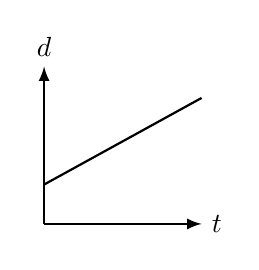
\begin{tikzpicture}
      \draw[thick,->](0,0)--(2,0)node[right]{$t$};
      \draw[thick,->](0,0)--(0,2)node[above]{$d$};
      \draw[thick,](0,.5)--(2,1.6);
    \end{tikzpicture}

    \choice
    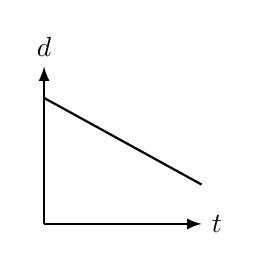
\begin{tikzpicture}
      \draw[thick,->](0,0)--(2,0)node[right]{$t$};
      \draw[thick,->](0,0)--(0,2)node[above]{$d$};
      \draw[thick,](0,1.6)--(2,.5);
    \end{tikzpicture}

    \choice
    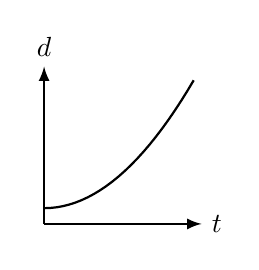
\begin{tikzpicture}
      \draw[thick,->](0,0)--(2,0)node[right]{$t$};
      \draw[thick,->](0,0)--(0,2)node[above]{$d$};
      \draw[thick,domain=0:1.9] plot(\x,{\x*\x*.45+.2});
    \end{tikzpicture}

    \choice
    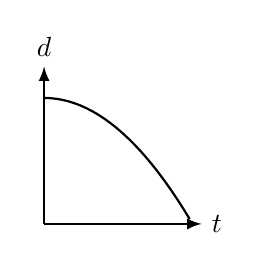
\begin{tikzpicture}
      \draw[thick,->](0,0)--(2,0)node[right]{$t$};
      \draw[thick,->](0,0)--(0,2)node[above]{$d$};
      \draw[thick,domain=0:1.85] plot(\x,{-\x*\x*.45+1.6});
    \end{tikzpicture}
  \end{oneparchoices}
  \vspace{.7in}
  
  \question A ball is thrown straight up from a point \SI{2}{\metre} above the
  ground. The ball reaches a maximum height of \SI{3}{\metre} above its
  starting point and then falls \SI5{\metre} to the ground. When the ball
  strikes the ground, what is its displacement from its starting point?

  \begin{oneparchoices}
    \choice Zero
    \choice 8 m below
    \choice 5 m below
    \choice 2 m below
    \choice 3 m above
  \end{oneparchoices}
  \vspace{.7in}
  
  \question What do acceleration and velocity have in common?
  \begin{choices}
    \choice Both are scalars.
    \choice Both are vectors.
    \choice Both are measured in units of distance divided by time.
    \choice Both are measured in units of distance divided by time squared.
    \choice They are different names for the same quantity.
  \end{choices}

  \question Two projectiles are launched with the same initial speed from the
  same location, one at a \ang{30} angle and the other at a \ang{60} angle with
  the horizontal. They land at the same height at which they were launched. If
  air resistance is negligible, how do the projectiles' respective maximum
  heights, $H_{30}$ and $H_{60}$ , and times in the air, $T_{30}$ and $T_{60}$,
  compare with each other?

  \begin{tabular}{ccc}
    & \underline{Maximum Height} & \underline{Time in Air} \\
    A. & $H_{30} > H_{60}$ & $T_{30} > T_{60}$ \\
    B. & $H_{30} > H_{60}$ & $T_{30} < T_{60}$ \\
    C. & $H_{30} = H_{60}$ & $T_{30} = T_{60}$ \\
    D. & $H_{30} < H_{60}$ & $T_{30} > T_{60}$ \\
    E. & $H_{30} < H_{60}$ & $T_{30} < T_{60}$
  \end{tabular}

  \question An object of mass \SI{100}{\kilo\gram} is initially at rest on a
  horizontal frictionless surface. At time $t=0$, a horizontal force of
  \SI{10}{\newton} is applied to the object for \SI{1}{\second} and then
  removed. Which of the following is true of the object at time
  $t=\SI{2}{\second}$ if it is still on the surface?
  \begin{choices}
    \choice It is at the same position it had at $t=0$, since a force of
    \SI{10}{\newton} is not large enough to move such a massive object.
    \choice It is moving with constant nonzero acceleration.
    \choice It is moving with decreasing acceleration.
    \choice It is moving at a constant velocity.
    \choice It has come to rest some distance away from the position it had at
    $t=0$.
  \end{choices}
  \vspace{.7in}
  
  \question Several forces act on an object, but the object is in equilibrium.
  Which of the following statements about the object must be true?
  \begin{enumerate}[nosep]
  \item[I.] It has zero acceleration.
  \item[II.] The net force acting on it is zero.
  \item[III.] It is at rest.
  \item[IV.] It is moving with constant velocity.
  \end{enumerate}

  \begin{oneparchoices}
    \choice I and II
    \choice I and III
    \choice I and IV
    \choice II and III
    \choice II and IV
  \end{oneparchoices}
  \newpage
  
  \fullwidth{
    \textbf{Question \ref{proj1}--\ref{proj2}}
    \begin{center}
      \pic{.45}{projectile1}
    \end{center}
    A rock is thrown from the edge of a cliff with an initial velocity $v_0$ at
    an angle $\theta$ with the horizontal as shown\\
    above. Point $P$ is the highest point in the rock's trajectory and point
    $Q$ is level with the starting point. Assume\\
    air resistance is negligible.
  }

  \question Which of the following correctly describes the horizontal and
  vertical speeds and the acceleration of the rock at point $P$?
  \label{proj1}

  \begin{tabular}{cccc}
    & Horizontal Speed & Vertical Speed & Acceleration \\ \hline
    (A)  & $v_0\cos\theta$ & 0 & $g$ \\
    (B)  & 0               & 0 & $g$ \\
    (C)  & $v_0\cos\theta$ & 0 & 0   \\
    (D)  & $v_0\cos\theta$ & $v_0\sin\theta$ & 0   \\
    (E)  & 0 & $v_0\cos\theta$ & 0
  \end{tabular}

  \question Which of the following correctly describes the horizontal and
  vertical speeds and the acceleration of the rock at point $Q$?
  \label{proj2}

  \begin{tabular}{cccc}
    & Horizontal Speed & Vertical Speed & Acceleration \\ \hline
    (A)  & $v_0\cos\theta$ & 0 & $g$ \\
    (B)  & 0               & 0 & $g$ \\
    (C)  & $v_0\cos\theta$ & 0 & 0   \\
    (D)  & $v_0\cos\theta$ & $v_0\sin\theta$ & 0   \\
    (E)  & 0 & $v_0\cos\theta$ & 0
  \end{tabular}

  \begin{center}
    \pic{.55}{child}
  \end{center}
  \question As shown in the figure above, a child of mass \SI{20}{\kilo\gram}
  who is running at a speed of \SI{4.}{\metre\per\second} jumps onto a
  stationary sled of mass \SI{5.}{\kilo\gram} on a frozen lake. The speed at
  which the child and sled begin to slide across the ice is most nearly

  \begin{oneparchoices}
    \choice \SI{.20}{\metre\per\second}
    \choice \SI{.80}{\metre\per\second}
    \choice \SI{1.2}{\metre\per\second}
    \choice \SI{3.2}{\metre\per\second}
    \choice \SI{16}{\metre\per\second}
  \end{oneparchoices}
  \vspace{.6in}
  
  \question A toy spacecraft is launched directly upward. When the toy reaches
  its highest point, a spring is released and the toy splits into two parts
  with masses of \SI{.02}{\kilo\gram} and \SI{.08}{\kilo\gram}, respectively.
  Immediately after the separation, the \SI{.02}{\kilo\gram} part moves
  horizontally due east. Air resistance is negligible. True statements about
  the \SI{.08}{\kilo\gram} part include which of the following?
  \begin{enumerate}[nosep]
  \item[I.] It could move north immediately after the spring is released.
  \item[II.] It takes longer to reach the ground than does the
    \SI{.02}{\kilo\gram} part.
  \item[III.] It strikes the ground farther from the launch point than does the
    \SI{.02}{\kilo\gram} part.
  \end{enumerate}
  \begin{oneparchoices}
    \choice None
    \choice I only
    \choice III only
    \choice I and II only
    \choice II and III only
  \end{oneparchoices}
  \vspace{.6in}
  
  \question A student initially stands on a circular platform that is free to
  rotate without friction about its center. The student jumps off tangentially,
  setting the platform spinning. Quantities that are conserved for the
  student-platform system as the student jumps include which of the following?
  \begin{enumerate}[nosep]
  \item[I.] Angular momentum
  \item[II.] Linear momentum
  \item[III.] Kinetic energy
  \end{enumerate}
  \begin{oneparchoices}
    \choice I only
    \choice II only
    \choice I and II only
    \choice II and III only
    \choice I, II, and III
  \end{oneparchoices}
  \vspace{.7in}
  \newpage
  
  \question In an experiment with a simple pendulum, measurements of the period
  $T$ of the pendulum are made for different values of its length $L$.
  When plotted on a graph, which of the following should result in a
  straight-line fit of the data?

  \begin{oneparchoices}
    \choice $\sqrt{T}$ versus $L$
    \choice $T$ versus $L$
    \choice $T$ versus $L^2$
    \choice $T^2$ versus $L$
    \choice $T^2$ versus $L^2$
  \end{oneparchoices}
  \vspace{.7in}

  \begin{center}
    \pic{.18}{comet}
  \end{center}
  \question A comet moves in the Sun's gravitational field, following the path
  shown above. What happens to its angular momentum as it moves from point $X$
  to point $Y$?
  \begin{choices}
    \choice It increases steadily.
    \choice It remains constant.
    \choice It decreases steadily.
    \choice It increases as it approaches the Sun and decreases as it moves
    away from the Sun.
    \choice It decreases as it approaches the Sun and increases as it moves
    away from the Sun.
  \end{choices}
  \vspace{.7in}

  \question Satellite $X$ moves around Earth in a circular orbit of radius $R$.
  Satellite $Y$ is also in a circular orbit around Earth, and it completes one
  orbit for every eight orbits completed by satellite $X$. What is the
  orbital radius of satellite $Y$?

  \begin{oneparchoices}
    \choice $\dfrac14R$\hspace{.2in}
    \choice $\dfrac12R$\hspace{.2in}
    \choice $2R$\hspace{.2in}
    \choice $4R$\hspace{.2in}
    \choice $8R$
  \end{oneparchoices}
  \vspace{.2in}

\item A newly discovered planet is found to have twice the radius and five
  times the mass of Earth. If the acceleration of gravity at the surface of
  Earth is $g$, the acceleration of gravity at the surface of the new planet is

  \begin{oneparchoices}
    \choice $\dfrac{2g}5$\hspace{.2in}
    \choice $\dfrac{4g}5$\hspace{.2in}
    \choice $g$\hspace{.2in}
    \choice $\dfrac{5g}4$\hspace{.2in}
    \choice $\dfrac{5g}2$
  \end{oneparchoices}
  \vspace{.2in}

  \fullwidth{
    \textbf{Questions \ref{toycar1}--\ref{toycar2}}
    
    A toy car of mass 6 kg, moving in a straight path, experiences a net force
    given by the function $F=-3t$. At time $t=0$, the car has a velocity of
    \SI{4}{\metre\per\second} in the positive direction and is located
    $+8$ m from the origin.
  }
  
  \question The car will come instantaneously to rest at time $t$ equal to

  \begin{oneparchoices}
    \choice$\dfrac23$ \si\second
    \choice$\sqrt{\dfrac43}$ \si\second
    \choice$\sqrt{\dfrac83}$ \si\second
    \choice$\sqrt8$ \si\second
    \choice\SI{4}{\second}
  \end{oneparchoices}
  \label{toycar1}

  \question Which of the following best shows a graph of position $d$ versus
  time $t$ for the car?
  
  \begin{oneparchoices}
    \choice
    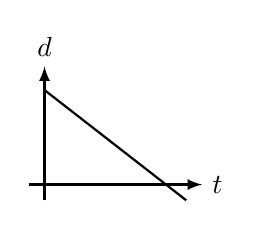
\begin{tikzpicture}
      \draw[thick,->](-.2,0)--(2,0)  node[right]{$t$};
      \draw[thick,->](0,-.2)--(0,1.5)node[above]{$d$};
      \draw[thick](0,1.2)--(1.8,-.2);
    \end{tikzpicture}

    \choice
    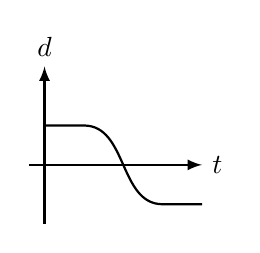
\begin{tikzpicture}
      \draw[thick,->](-.2,0)--(2,0)  node[right]{$t$};
      \draw[thick,->](0,-.75)--(0,1.25)node[above]{$d$};
      \draw[thick] (0,.5)--(.5,.5) to [out=0,in=180](1.5,-.5)--(2,-.5);
    \end{tikzpicture}

    \choice
    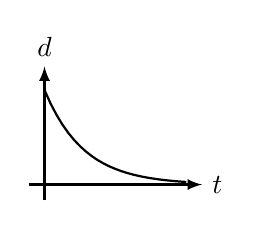
\begin{tikzpicture}
      \draw[thick,->](-.2,0)--(2,0)  node[right]{$t$};
      \draw[thick,->](0,-.2)--(0,1.5)node[above]{$d$};
      \draw[thick,domain=0:1.8]plot(\x,{1.2*exp(-2*\x)});
    \end{tikzpicture}
    
    \choice
    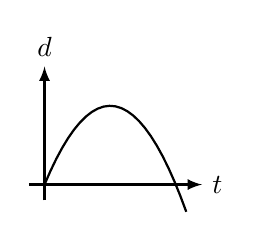
\begin{tikzpicture}
      \draw[thick,->](-.2,0)--(2,0)  node[right]{$t$};
      \draw[thick,->](0,-.2)--(0,1.5)node[above]{$d$};
      \draw[thick,domain=0:1.8]plot(\x,{-4*(.6*\x-.5)*(.6*\x-.5)+1});

    \end{tikzpicture}

    \choice
    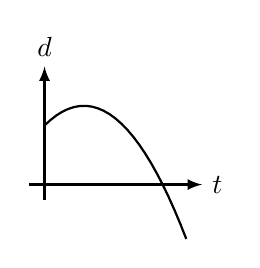
\begin{tikzpicture}
      \draw[thick,->](-.2,0)--(2,0)  node[right]{$t$};
      \draw[thick,->](0,-.2)--(0,1.5)node[above]{$d$};
      \draw[thick,domain=0:1.8]plot(\x,{-(\x-.5)*(\x-.5)+1});
    \end{tikzpicture}
  \end{oneparchoices}
  \label{toycar2}
  \vspace{.7in}
  \newpage
  
  \fullwidth{
    \textbf{Questions \ref{connect1}--\ref{connect2}}
    \begin{center}
      \pic{.3}{connected-mass}
    \end{center}
    A block of mass $M_1$ on a horizontal table is connected to a hanging block
    of mass $M_2$ by a string that passes over a pulley, as shown above. The
    acceleration of the blocks is $0.6g$. Assume that friction and the mass of
    the string are negligible.
  }

  \question The tension $T$ in the string is \label{connect1}
  
  \begin{oneparchoices}
    \choice zero
    \choice $0.4M_2g$
    \choice $0.6M_2g$
    \choice $1.0M_2g$
    \choice $1.6M_2g$
  \end{oneparchoices}
  \vspace{.2in}
  
  \question The ratio of masses $M_2/M_1$ is  \label{connect2}
   
  \begin{oneparchoices}
    \choice 0.67
    \choice 1.0
    \choice 1.4
    \choice 1.5
    \choice 1.6
  \end{oneparchoices}
  \vspace{.2in}

  \fullwidth{
    \textbf{Questions \ref{spring1}--\ref{spring2}}
    \begin{center}
      \pic{.4}{spring-mass}
    \end{center}
    In the system of two blocks and a spring shown above, blocks 1 and 2 are
    connected by a string that passes over a pulley. The initially unstretched
    spring connects block 1 to a rigid wall. Block 1 is released from rest,
    initially slides to the right, and is eventually brought to rest by the
    spring and by friction on the horizontal surface.
  }

  \question Which of the following is true of the energy of the system during
  this process?
  \begin{choices}
    \choice The total mechanical energy of the system is conserved.
    \choice The total mechanical energy of the system increases.
    \choice The energy lost to friction is equal to the gain in the potential
    energy of the spring.
    \choice  The potential energy lost by block 2 is less in magnitude than the
    potential energy gained by the spring.
    \choice The potential energy lost by block 2 is greater in magnitude than
    the potential energy gained by the spring.
  \end{choices}
  \label{spring1}
  \vspace{.7in}

  \question After block 1 comes to rest, the force exerted on it by the spring
  must be equal in magnitude to
  \begin{choices}
    \choice zero
    \choice the frictional force on block 1
    \choice the vector sum of the forces on block 1 due to friction and tension
    in the string
    \choice the sum of the weights of the two blocks
    \choice the difference in the weights of the two blocks
  \end{choices}
  \label{spring2}

  \begin{center}
    \pic{.25}{impulse}
  \end{center}
  \question The graph above shows the force acting on an object as a function
  of time. The change in momentum of the object from time 0 to $t$ is

  \begin{oneparchoices}
    \choice $2Ft$\hspace{.3in}
    \choice $Ft$\hspace{.3in}
    \choice $\dfrac12Ft$\hspace{.3in}
    \choice $\dfrac14Ft$\hspace{.3in}
    \choice zero
  \end{oneparchoices}

  \fullwidth{
    \textbf{Questions \ref{orbit1}--\ref{orbit2}}
    \begin{center}
      \pic{.4}{orbit}\\
      \underline{Note:} Figure not drawn to scale.
    \end{center}
    A moon of mass $m$ orbits a planet of mass $49m$ in an elliptical orbit as
    shown above. When the moon is at point $A$, its distance from the center of
    the planet is $r_A$ and its speed is $v_0$. When the moon is at point $B$,
    its speed is $5u_0$.
  }

  \question When the moon is at point $A$, the distance from the moon to the
  center of mass of the planet-moon system is most nearly

  \begin{oneparchoices}
    \choice $\dfrac1{50}r_A$
    \choice $\dfrac17r_A$
    \choice $\dfrac12r_A$
    \choice $\dfrac67r_A$
    \choice $\dfrac{49}{50}r_A$
  \end{oneparchoices}
  \label{orbit1}
  \vspace{.2in}
  
  \question When the moon is at point $B$, the distance from the moon to the
  center of the planet is most nearly

  \begin{oneparchoices}
    \choice $\dfrac1{25}r_A$
    \choice $\dfrac15r_A$
    \choice $\dfrac1{\sqrt5}r_A$
    \choice $r_A$
    \choice $\sqrt5r_A$
  \end{oneparchoices}
  \label{orbit2}
  \vspace{.2in}

  \fullwidth{
    \textbf{Questions \ref{beam1}--\ref{beam2}}
    \begin{center}
      \pic{.22}{beam}
    \end{center}
    The bar shown above is pivoted about one end and is initially at rest in a
    vertical position. The bar is displaced slightly and as it falls it makes
    an angle $\theta$ with the vertical at any given time, as shown above.
  }
  \question Which of the following graphs best represents the bar's angular
  acceleration a as a function of angle $\theta$?

  \begin{oneparchoices}
    \choice
    \begin{tikzpicture}
      \draw[thick,->](0,0)--(2,0)node[right]{$\theta$};
      \draw[thick,->](0,0)--(0,2)node[above]{$\alpha$};
      \draw[thick](0,1)--(1.8,1);
    \end{tikzpicture}

    \choice
    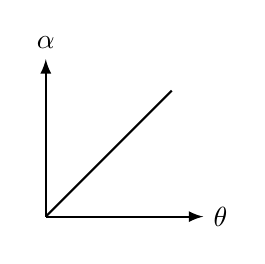
\begin{tikzpicture}
      \draw[thick,->](0,0)--(2,0)node[right]{$\theta$};
      \draw[thick,->](0,0)--(0,2)node[above]{$\alpha$};
      \draw[thick](0,0)--(1.6,1.6);
    \end{tikzpicture}

    \choice
    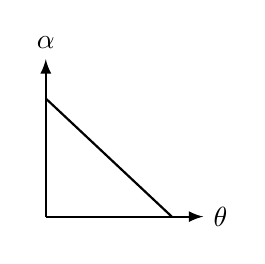
\begin{tikzpicture}
      \draw[thick,->](0,0)--(2,0)node[right]{$\theta$};
      \draw[thick,->](0,0)--(0,2)node[above]{$\alpha$};
      \draw[thick](0,1.5)--(1.6,0);
    \end{tikzpicture}

    \choice
    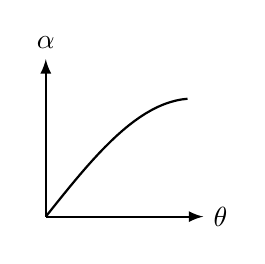
\begin{tikzpicture}
      \draw[thick,->](0,0)--(2,0)node[right]{$\theta$};
      \draw[thick,->](0,0)--(0,2)node[above]{$\alpha$};
      \draw[thick,domain=0:1.8]plot(\x,{1.5*sin(48*\x)});
    \end{tikzpicture}

    \choice
    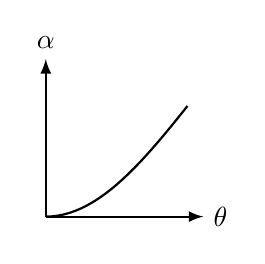
\begin{tikzpicture}
      \draw[thick,->](0,0)--(2,0)node[right]{$\theta$};
      \draw[thick,->](0,0)--(0,2)node[above]{$\alpha$};
      \draw[thick,domain=0:1.8]plot(\x,{-1.5*cos(48*\x)+1.5});
    \end{tikzpicture}
  \end{oneparchoices}
  \label{beam1}
  \vspace{.7in}
  
  \question Which of the following graphs best represents the bar's angular
  velocity $\omega$ as a function of time?

  \begin{oneparchoices}
    \choice
    \begin{tikzpicture}
      \draw[thick,->](0,0)--(2,0)node[right]{$\theta$};
      \draw[thick,->](0,0)--(0,2)node[above]{$\omega$};
      \draw[thick](0,1)--(1.8,1);
    \end{tikzpicture}

    \choice
    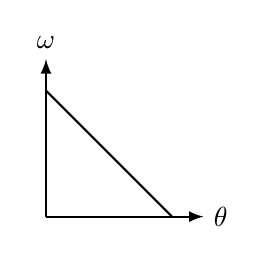
\begin{tikzpicture}
      \draw[thick,->](0,0)--(2,0)node[right]{$\theta$};
      \draw[thick,->](0,0)--(0,2)node[above]{$\omega$};
      \draw[thick](0,1.6)--(1.6,0);
    \end{tikzpicture}

    \choice
    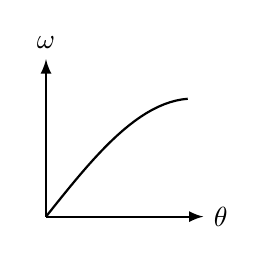
\begin{tikzpicture}
      \draw[thick,->](0,0)--(2,0)node[right]{$\theta$};
      \draw[thick,->](0,0)--(0,2)node[above]{$\omega$};
      \draw[thick,domain=0:1.8]plot(\x,{1.5*sin(48*\x)});
    \end{tikzpicture}

    \choice
    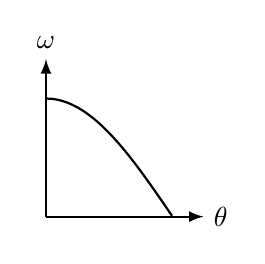
\begin{tikzpicture}
      \draw[thick,->](0,0)--(2,0)node[right]{$\theta$};
      \draw[thick,->](0,0)--(0,2)node[above]{$\omega$};
      \draw[thick,domain=0:1.6]plot(\x,{1.5*cos(56*\x)});
    \end{tikzpicture}

    \choice
    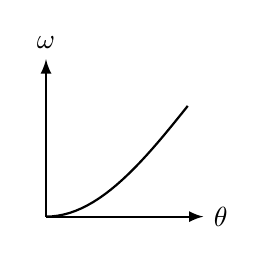
\begin{tikzpicture}
      \draw[thick,->](0,0)--(2,0)node[right]{$\theta$};
      \draw[thick,->](0,0)--(0,2)node[above]{$\omega$};
      \draw[thick,domain=0:1.8]plot(\x,{-1.5*cos(48*\x)+1.5});
    \end{tikzpicture}
  \end{oneparchoices}
  \label{beam2}
  \vspace{.7in}
  \begin{center}
    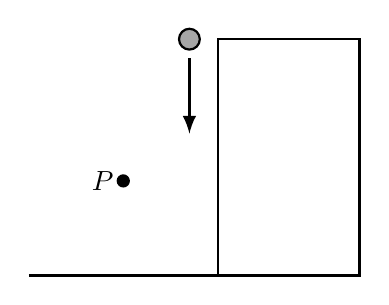
\begin{tikzpicture}[scale=1.2]
      \draw[thick](0,0)--(2,0);
      \draw[thick](2,0) rectangle(3.5,2.5);
      \fill(1,1) circle(.07) node[left]{$P$};
      \draw[thick,fill=gray!70](1.7,2.5) circle(.11);
      \draw[very thick,->](1.7,2.3)--(1.7,1.5);
    \end{tikzpicture}
  \end{center}
  \question A stone falls from rest from the top of a building as shown above.
  Which of the following graphs best represents the stone's angular momentum $L$
  about the point $P$ as a function of time?

 \begin{oneparchoices}
    \choice
    \begin{tikzpicture}
      \draw[thick,->](0,0)--(2,0)node[right]{$t$};
      \draw[thick,->](0,0)--(0,2)node[above]{$L$};
      \draw[ultra thick](0,0)--(1.8,0);
    \end{tikzpicture}

    \choice
    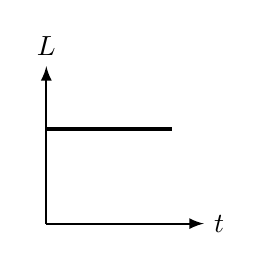
\begin{tikzpicture}
      \draw[thick,->](0,0)--(2,0)node[right]{$t$};
      \draw[thick,->](0,0)--(0,2)node[above]{$L$};
      \draw[ultra thick](0,1.2)--(1.6,1.2);
    \end{tikzpicture}

    \choice
    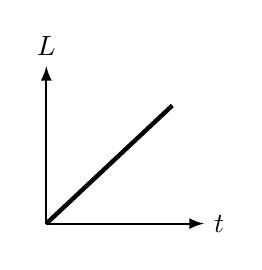
\begin{tikzpicture}
      \draw[thick,->](0,0)--(2,0)node[right]{$t$};
      \draw[thick,->](0,0)--(0,2)node[above]{$L$};
      \draw[ultra thick](0,0)--(1.6,1.5);
    \end{tikzpicture}

    \choice
    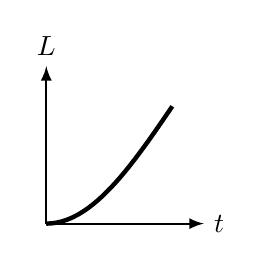
\begin{tikzpicture}
      \draw[thick,->](0,0)--(2,0)node[right]{$t$};
      \draw[thick,->](0,0)--(0,2)node[above]{$L$};
      \draw[ultra thick,domain=0:1.6]plot(\x,{-1.5*cos(56*\x)+1.5});
    \end{tikzpicture}

    \choice
    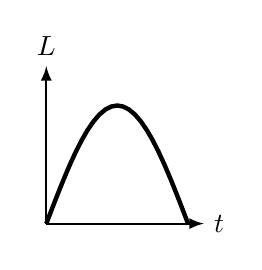
\begin{tikzpicture}
      \draw[thick,->](0,0)--(2,0)node[right]{$t$};
      \draw[thick,->](0,0)--(0,2)node[above]{$L$};
      \draw[ultra thick,domain=0:1.8]plot(\x,{1.5*sin(100*\x)});
    \end{tikzpicture}
  \end{oneparchoices}
  
  %    %\vspace{\stretch1}
%    \columnbreak
%  
%    \question A golf ball is hit from level ground and has a horizontal range of
%    \SI{100}\metre. The ball leaves the golf club at an angle of \ang{60} to
%    the level ground. At what other angle(s) can the ball be struck at the same
%    initial velocity and still have a range of \SI{100}{\metre}?
%    \cpic{.25}{golf-ball}
%    \begin{choices}
%      \choice\ang{30}
%      \choice\ang{20} and \ang{80}
%      \choice\ang{10} and \ang{120}
%      \choice\ang{45} and \ang{135}
%      \choice There is no other angle other than \ang{60} in which the ball will
%      have a range of \SI{100}{\metre}.
%    \end{choices}
%%TML\vspace{.7in}
%
%    \fullwidth{\textbf{Questions \ref{q:particle1}--\ref{q:particle2}}
%    
%      A particle moves on a horizontal surface with a constant acceleration of
%      \SI{6}{\metre\per\second\squared} in the $x$-direction and
%      \SI{4}{\metre\per\second\squared} in the $y$-direction. The initial
%      velocity of the particle is \SI3{\metre\per\second} in the $x$-direction.
%    }
%
%    \question The speed of the particle after \SI{4}{\second} is
%    \begin{choices}
%      \choice\SI{16 }{\metre\per\second}
%      \choice\SI{27 }{\metre\per\second}
%      \choice\SI{31 }{\metre\per\second}
%      \choice\SI{44 }{\metre\per\second}
%      \choice\SI{985}{\metre\per\second}
%    \end{choices}
%    \label{q:particle1}
%    
%    \question The displacement of the particle from its initial position is
%    \begin{choices}
%      \choice\SI{16}{\metre}
%      \choice\SI{32}{\metre}
%      \choice\SI{60}{\metre}
%      \choice\SI{68}{\metre}
%      \choice\SI{92}{\metre}
%    \end{choices}
%    \label{q:particle2}
%    
%    \question A rubber ball is dropped from rest onto a plane angled at
%    $\theta=\ang{30}$ to the horizontal floor and bounces off the plane with a
%    horizontal speed $v_0$. The ball lands on the plane a distance $D$ along the
%    plane, as shown below. In terms of $v_0$, $D$, and $g$, the speed of the
%    ball just before striking the plane is
%    \cpic{.23}{bounce}
%    \begin{choices}
%      \choice $v_0$
%      \choice $\displaystyle\left(v_0^2+2D\sin\theta g\right)^\frac{1}{2}$
%      \choice $\displaystyle\left(v_0+\frac{D\sin\theta}{g}\right)^\frac{1}{2}$
%      \choice $\displaystyle\left(v_0^2+\frac{D\sin\theta}{g}\right)^\frac{1}{2}$
%      \choice $\displaystyle\left(2D\sin\theta g\right)^\frac{1}{2}$
%    \end{choices}
%    \vspace{.7in}
%    \columnbreak
%  
%    \question A stack of coffee filters falls from rest through the air. Due to
%    air resistance, the filters fall with an acceleration proportional to the
%    velocity of fall, that is, $a=-kv$, where $k$ is a positive constant. The
%    velocity of the falling filters as a function of time of fall is
%    \begin{choices}
%      \choice $-kv^2$
%      \choice $-1⁄2kv^2$
%      \choice $-k$
%      \choice $\ln(kt)$
%      \choice $v_0e^{-kt}$
%    \end{choices}
%    
%    \question A small ball is launched with a speed of \SI{8}{m/s} at an angle
%    of \ang{30} from the horizontal. A cup is hung so that it is in position to
%    catch the ball when it reaches its maximum height. How far above the floor
%    should the cup be hung to catch the ball?    
%    \cpic{.3}{cup}
%    \begin{choices}
%      \choice\SI{2.4}{\metre}
%      \choice\SI{1.6}{\metre}
%      \choice\SI{1.0}{\metre}
%      \choice\SI{.8}{\metre}
%      \choice\SI{.4}{\metre}
%    \end{choices}
%  
%    \question The velocity vs.\ time graph below represents the motion of a
%    bicycle rider. The displacement of the rider between $0$ and \SI{4}{\hour}
%    is
%    \begin{center}
%      \begin{tikzpicture}[xscale=.8,yscale=.05]
%        \draw[thick,->](0,0)--(4.4,0) node[right]{\footnotesize $t$ (h)};
%        \draw[thick,->](0,-22)--(0,25)node[above]{\footnotesize $v$ (km/h)};
%        \foreach\x in {1,...,4}
%        \draw(\x,2)--(\x,-2)node[below]{\footnotesize\x};
%        \foreach\y in {-20,-10,...,20}
%        \draw(.1,\y)--(-.1,\y)node[left]{\footnotesize\y};
%        \draw[very thick](0,0)--(1,20)--(2,20)--(3,0)--(4,-20);
%        \draw[dotted](1,0)--(1,20);
%        \draw[dotted](2,0)--(2,20);
%      \draw[dotted](4,0)--(4,-20);
%      \end{tikzpicture}
%    \end{center}
%    \begin{choices}
%      \choice $+\SI{10}{\kilo\metre}$
%      \choice $+\SI{20}{\kilo\metre}$
%      \choice $+\SI{30}{\kilo\metre}$
%      \choice $+\SI{40}{\kilo\metre}$
%      \choice $-\SI{10}{\kilo\metre}$
%    \end{choices}
%
%    \fullwidth{
%      \textbf{Questions \ref{car1}--\ref{car2}}
%      
%      A car of mass $m$ travels along a straight horizontal road. The car begins
%      with a speed $v_0$, but accelerates according to the velocity function
%      $\displaystyle v=\left(v_0^2+\frac{Ct^2}{m}\right)$, where $t$ is time.
%    }
%
%    \question The speed of the car is zero at a time $t$ of
%    \begin{choices}
%      \choice zero
%      \choice $2t$
%      \choice $4t$
%      \choice $\sqrt{8t}$
%      \choice The speed of the car is never zero.
%    \end{choices}
%    \vspace{.7in}
%    \label{car1}
%    
%    \question The acceleration of the car as a function of time is
%    \begin{choices}
%      \choice $\displaystyle\left(v_0^2+\frac{Ct^2}{m}\right)$
%      \choice $\displaystyle\left(v_0^2+\frac{2Ct^2}{m}\right)$
%      \choice $\displaystyle\left(v_0+\frac{Ct}{m}\right)$
%      \choice $\displaystyle\left(\frac{2Ct}{m}\right)$
%      \choice $\displaystyle\left(\frac{2Ct^2}{m}\right)$
%    \end{choices}
%    \label{car2}
%    \columnbreak
%  
%    \fullwidth{
%      \textbf{Questions \ref{q:graph1}--\ref{q:graph2}}
%      
%      The graph shown below represents the velocity vs.\ time graphs for two
%      cars, $P$ and $Q$. Car $P$ begins with a speed $v_P$, and Car $Q$ begins
%      with a speed $v_Q$ which is twice the velocity of Car $P$, that is,
%      $v_Q=2v_P$. Both car starts at the same position at $t=0$.
%    
%      \begin{center}
%        \begin{tikzpicture}[scale=.5]
%          \draw[thick,->](0,0)--(5,0) node[right]{$t$};
%          \draw[thick,->](0,0)--(0,5) node[above]{$v$};
%          \draw[ultra thick](0,4)--(4,0);
%          \draw[ultra thick](0,2)--(4,2);
%          \draw[thick](2,.2)--(2,-.2) node[below]{10};
%          \draw[thick](4,.2)--(4,-.2) node[below]{20};
%          \draw[thick](.2,4)--(-.2,4) node[left]{$v_Q$};
%          \draw[thick](.2,2)--(-.2,2) node[left]{$v_P$};
%        \end{tikzpicture}
%      \end{center}
%    }
%    
%    \question Which of the following is true at a time of \SI{10}{\second}?
%    \begin{choices}
%      \choice The cars occupy the same position.
%      \choice Car $P$ is at rest.
%      \choice $v_Q>v_P$
%      \choice $v_P>v_Q$
%      \choice Car $Q$ is ahead of Car $P$.
%    \end{choices}
%    \label{q:graph1}
%    \vspace{.7in}
%    
%    \question Which of the following is true at a time of \SI{20}{\second}?
%    \begin{choices}
%      \choice The cars occupy the same position.
%      \choice Car $P$ is at rest.
%      \choice $v_Q>v_P$
%      \choice $a_P=a_Q$
%      \choice\ Car $P$ is ahead of Car $Q$.
%    \end{choices}
%    \label{q:graph2}
%    \vspace{.7in}
%    
%    \question A car is initially moving with a positive velocity of \SI{20}{m/s}
%    when it passes the origin at time $t=0$. The car continues to move at
%    \SI{20}{\metre\per\second} between $t=0$ and $t=\SI{2}{\second}$. At
%    $t=\SI{2}{\second}$, the driver presses the brake, giving the car an
%    acceleration of \SI{-4}{\metre\per\second^2}. The displacement of the car
%    at $t=\SI{6}{\second}$ is
%    \begin{choices}
%      \choice\SI{40}{\metre}
%      \choice\SI{32}{\metre}
%      \choice\SI{48}{\metre}
%      \choice\SI{64}{\metre}
%      \choice\SI{88}{\metre}
%    \end{choices}
%  
%    \question Which of the following pairs of graphs could show the position
%    vs.\ time and velocity vs.\ time graphs for the acceleration vs. time graph
%    shown above? Assume $v=0$ and $x=0$ at $t=0$.
%    \begin{center}
%      \begin{tikzpicture}[scale=.5]
%        \draw[thick,->](0,0)--(8,0) node[right]{$t$};
%        \draw[thick,->](0,-3)--(0,3) node[above]{$a$};
%        \draw[ultra thick](0,2)--(2,2);
%        \draw[ultra thick](2,0)--(4,0);
%        \draw[ultra thick](4,-2)--(6,-2);
%        \draw[ultra thick](6,0)--(8,0);
%        \draw[thick,dashed](2,2)--(2,0);
%        \draw[thick,dashed](4,0)--(4,-2);
%        \draw[thick,dashed](6,0)--(6,-2);
%      \end{tikzpicture}
%    \end{center}
%    \pic{.5}{xt-vt}
%    %\vspace{.7in}
%    \columnbreak
%  
%    \question A small airplane can fly at \SI{200}{km/h} with no wind. The pilot
%    of the plane would like to fly to a destination \SI{100}{km} due north of
%    his present position, but there is a crosswind of \SI{50}{km/h} east. How
%    much time is required for the plane to fly north to its destination?
%    \begin{choices}
%      \choice less than \SI{1/2}{\hour}
%      \choice \SI{1/2}{\hour}
%      \choice more than \SI{1/2}{\hour}
%      \choice \SI1\hour
%      \choice more than \SI1\hour
%    \end{choices}
%    \vspace{.7in}
%    
%    \question Two velocity vectors $v_1$ and $v_2$ each have a magnitude of
%    \SI{10}{\metre\per\second}. Graph 1 shows the velocity $v_1$ at
%    $t=\SI{0}{\second}$, and then the same object has a velocity $v_2$ at
%    $t=\SI{2}{\second}$, shown in Graph 2. Which of the following vectors best
%    represents the average acceleration vector that causes the object's velocity
%    to change from $v_1$ to $v_2$ ?
%    \begin{center}
%      \begin{tikzpicture}[scale=.5]
%        \draw[thick](-2,0)--(2,0);
%        \draw[thick](0,-2)--(0,2) node[pos=0,below]{Graph 1};
%        \draw[ultra thick,->](0,0)--(1.5,0) node[above]{$v_1$};
%      \end{tikzpicture}
%      \hspace{.2in}
%      \begin{tikzpicture}[scale=.5]
%        \draw[thick](-2,0)--(2,0);
%        \draw[thick](0,-2)--(0,2) node[pos=0,below]{Graph 2};
%        \draw[ultra thick,->](0,0)--(0,1.5) node[right]{$v_2$};
%      \end{tikzpicture}
%    \end{center}
%    \begin{choices}
%      \choice
%      \begin{tikzpicture}[scale=.5]
%        \draw[thick](-2,0)--(2,0);
%        \draw[thick](0,0)--(0,2);
%        \draw[ultra thick,->](0,0)--(0,1.5);
%      \end{tikzpicture}
%      \choice
%      \begin{tikzpicture}[scale=.5]
%        \draw[thick](-2,0)--(2,0);
%        \draw[thick](0,0)--(0,2);
%        \draw[ultra thick,->](0,0)--(1.5,0);
%      \end{tikzpicture}
%      \choice
%      \begin{tikzpicture}[scale=.5]
%        \draw[thick](-2,0)--(2,0);
%        \draw[thick](0,0)--(0,2);
%        \draw[ultra thick,->](0,0)--(-1.5,0);
%      \end{tikzpicture}
%      \choice
%      \begin{tikzpicture}[scale=.5]
%        \draw[thick](-2,0)--(2,0);
%        \draw[thick](0,0)--(0,2);
%        \draw[ultra thick,->](0,0)--(1.12,1.12);
%      \end{tikzpicture}
%      \choice
%      \begin{tikzpicture}[scale=.5]
%        \draw[thick](-2,0)--(2,0);
%        \draw[thick](0,0)--(0,2);
%        \draw[ultra thick,->](0,0)--(-1.12,1.12);
%      \end{tikzpicture}
%    \end{choices}
%
%    \question An object starts from rest at $t=0$ and position $x=0$, then moves
%    in a straight line with an acceleration described by the equation $a=4t^2$
%    in \si{m/s^2}. What is the position of the object at $t=\SI{3}{\second}$?
%    \begin{choices}
%      \choice\SI{6}{\metre}
%      \choice\SI{1}{\metre}
%      \choice\SI{27}{\metre}
%      \choice\SI{54}{\metre}
%      \choice\SI{108}{\metre}
%    \end{choices}
%  
%    \question A ball is dropped from rest from the top of a cliff $80$ meters
%    high. At the same time, a rock is thrown horizontally from the top of the
%    same cliff. The rock and ball hit the level ground below a distance of
%    \SI{40}{\metre} apart. The horizontal velocity of the rock that was thrown
%    was most nearly
%    \begin{center}
%      \vspace{-.15in}\pic{.25}{ball-cliff}
%    \end{center}
%    \begin{choices}
%      \choice\SI{5}{\metre\per\second}
%      \choice\SI{10}{\metre\per\second}
%      \choice\SI{20}{\metre\per\second}
%      \choice\SI{40}{\metre\per\second}
%      \choice\SI{80}{\metre\per\second}
%    \end{choices}
%    
%%  \item A stone is dropped near the surface of Mars and falls with an
%%    acceleration of \SI{3.8}{m/s^2}. This means that the
%%    \begin{choices}
%%    \item distance the stone falls increases 3.8 meters for each second of
%%      fall
%%    \item derivative of the distance fallen with respect to time is
%%      \SI{3.8}{m/s}
%%    \item derivative of the velocity with respect to time is \SI{3.8}{m/s^2}
%%    \item velocity is constant at \SI{3.8}{m/s}
%%    \item derivative of the acceleration is \SI{3.8}{m/s^2}
%%    \end{choices}
%%    \vspace{.7in}
%%    
%%  \item A \SI{600}{\kilo\gram} car accelerates uniformly from rest. After
%%    \SI{4}{\second}, it reaches a speed of \SI{24}{m/s}. During the
%%    \SI{4}{\second}, the car has traveled a distance of
%%    \begin{choices}
%%    \item\SI{12}{\metre}
%%    \item\SI{24}{\metre}
%%    \item\SI{36}{\metre}
%%    \item\SI{48}{\metre}
%%    \item\SI{96}{\metre}
%%    \end{choices}
%      
%%  \item A passenger on a train moving horizontally at a constant speed relative
%%    to the ground drops a ball from his window. A stationary observer on the
%%    ground sees the ball falling with a speed $v_1$ at an angle to the vertical
%%    at the instant it is dropped from the train window, but the ball appears to
%%    be falling vertically with a speed $v_2$ at the same instant as viewed by
%%    the train passenger. What is the speed (magnitude of velocity) of the train
%%    relative to the ground after the ball is dropped? Neglect air resistance.
%%    \begin{choices}
%%    \item $ v_1 + v_2$
%%    \item $ v_1 - v_2$
%%    \item $ v_1^2 + v_2^2$
%%    \item $ v_1^2 - v_2^2$
%%    \item $\sqrt{v_1^2 - v_2^2}$
%%    \end{choices}
%    
%    \question A ball is hit straight up into the air with an upward positive
%    velocity. Wich of the following describes the velocity and acceleration
%    of the ball at the instant it reaches the top of its flight?
%  
%    \begin{tabular}{lcc}
%      & Velocity & Acceleration\\ \hline
%      (A) & $0$ & $0$\\
%      (B) & $0$ & $g$\\
%      (C) & $2v_0$ & $g$\\
%      (D) & $\frac12v_0$ & $0$\\
%      (E) & $0$ & $\frac12g$
%    \end{tabular}
%    \vspace{.7in}
%    \columnbreak
%  
%    \question A toy dart gun fires a dart at an angle of \ang{45} to the
%    horizontal and the dart reaches a maximum height of 1 meter. If the dart
%    were fired straight up into the air along the vertical, the dart would
%    reach a height of
%    \begin{choices}
%      \choice\SI1\metre
%      \choice\SI2\metre
%      \choice\SI3\metre
%      \choice\SI4\metre
%      \choice\SI5\metre
%    \end{choices}
%    
%    \question The graph below shows the displacement as a function of time for a
%    car moving in a straight line. Which of the following graphs shows the
%    velocity vs.\ time graph for the same time intervals?
%    \begin{center}
%      \pic{.25}{xt}
%    \end{center}
%    \pic{.3}{ab}\\
%    \pic{.38}{cde}
%    \newpage
%  
%    \fullwidth{
%      \textbf{Questions \ref{q:fall1}--\ref{q:fall2}}
%
%      An object is released from rest and falls through a resistive medium. The
%      resistance causes the velocity of the object to change according to the
%      equation $v=16t-\frac12t^4$, where $v$ is in \si{m/s} and time is in
%      \si{\second}.
%    }
%
%    \question Which of the following is a possible equation for the
%    acceleration of the object as a function of time?
%    \begin{choices}
%      \choice $16-2t^2$
%      \choice $16-2t^3$
%      \choice $16-2t$
%      \choice $8t^3-2t^2$
%      \choice $32t^3-2t^5$
%    \end{choices}
%    \label{q:fall1}
%    
%    \question What is the terminal velocity of the object as it falls?
%    \begin{choices}
%      \choice \SI{5 }{\metre\per\second}
%      \choice \SI{10}{\metre\per\second}
%      \choice \SI{24}{\metre\per\second}
%      \choice \SI{32}{\metre\per\second}
%      \choice The object never reaches a terminal velocity.
%    \end{choices}
%    \label{q:fall2}
%    \vspace{.7in}
%  
%    \question A student jumps off a cliff with an initial horizontal velocity
%    $v$ and lands in a lake below at a distance of $x$ from the base of the
%    cliff. In terms of his initial velocity $v$, how fast would he have had to
%    jump to land a distance $2x$ from the base of the cliff?
%    \begin{center}
%      \begin{tikzpicture}[scale=.5]
%        \draw[thick](0,4)--(0,0)--(6,0);
%        \draw[thick,->](0,4.2)--(1,4.2) node[right]{$v$};
%        \draw[fill=gray,thick] (0,4.2) circle(.1);
%        \draw[thick](2,.2)--(2,-.2) node[below]{$x$};
%        \draw[thick](4,.2)--(4,-.2) node[below]{$2x$};
%      \end{tikzpicture}
%    \end{center}
%    \begin{choices}
%      \choice $\sqrt{2v}$
%      \choice $2v$
%      \choice $4v$
%    \choice $8v$
%    \choice $16v$
%    \end{choices}
%    
%    \question An astronaut drops a hammer on a moon with no atmosphere. The
%    hammer falls a distance of $2$ meters in the first second. What is the
%    acceleration due to gravity on this moon?
%    \begin{choices}
%      \choice\SI{1}{\metre\per\second\squared}
%      \choice\SI{2}{\metre\per\second\squared}
%      \choice\SI{3}{\metre\per\second\squared}
%      \choice\SI{4}{\metre\per\second\squared}
%      \choice\SI{8}{\metre\per\second\squared}
%    \end{choices}
%
%    \question The motion of an object is represented by the acceleration vs.\
%    time graph below. The object begins from rest. Which of the following
%    statements is true about the motion of the object?
%    \begin{center}
%      \begin{tikzpicture}[scale=.5]
%        \draw[thick,->](0,0)--(6.3,0) node[right]{$t$};
%        \draw[thick,->](0,-3.5)--(0,3.5) node[above]{$a$};
%        \draw[ultra thick](0,2)--(2,2);
%        \draw[ultra thick](2,-2)--(4,-2);
%        \draw[dashed,thick](2,2)--(2,-2);
%        \draw[thick](2,.2)--(2,-.2) node[below]{2};
%        \draw[thick](4,.2)--(4,-.2) node[below]{4};
%        \draw[thick](.2,2)--(-.2,2) node[left]{+2};
%        \draw[thick](.2,-2)--(-.2,-2) node[left]{-2};
%      \end{tikzpicture}
%    \end{center}
%    \begin{choices}
%      \choice The object returns to its original position.
%      \choice The velocity of the object is zero at a time of \SI{2}{\second}.
%      \choice The velocity of the object is zero at a time of \SI{4}{\second}.
%      \choice The displacement of the object is zero at a time of \SI4{\second}.
%      \choice The acceleration of the object is zero at a time of \SI2{\second}.
%    \end{choices}
%  \end{questions}
%\end{multicols*}
%\newpage
%`
%%\begin{center}
%%  {\Large
%%    \textbf{AP\textsuperscript{\textregistered} Physics 1 \&C: Kinematics\\
%%      Student Answer Sheet for Multiple-Choice Section}
%%  }
%%  
%%  \begin{minipage}[t]{.3\textwidth}
%%  \vspace{.2in}
%%  \bgroup
%%  \begin{tabular}{>{\centering}m{1.3cm} >{\centering}m{1.7cm}}
%%    No. & Answer
%%  \end{tabular}\\
%%  \def\arraystretch{1.5}
%%  \begin{tabular}{|>{\centering}m{1.3cm}|>{\centering}m{1.7cm}|}
%%    \hline
%%    1 & \\ \hline
%%    2 & \\ \hline
%%    3 & \\ \hline
%%    4 & \\ \hline
%%    5 & \\ \hline
%%    6 & \\ \hline
%%    7 & \\ \hline
%%    8 & \\ \hline
%%    9 & \\ \hline
%%    10 & \\ \hline
%%    11 & \\ \hline
%%    12 & \\ \hline
%%    13 & \\ \hline
%%    14 & \\ \hline
%%    15 & \\ \hline
%%    16 & \\ \hline
%%    17 & \\ \hline
%%    18 & \\ \hline
%%    19 & \\ \hline
%%    20 & \\ \hline
%%    21 & \\ \hline
%%    22 & \\ \hline
%%    23 & \\ \hline
%%    24 & \\ \hline
%%    25 & \\ \hline
%%  \end{tabular}
%%  \egroup
%%  \end{minipage}
%%  \begin{minipage}[t]{.3\textwidth}
%%  \vspace{.2in}
%%  \bgroup
%%  \begin{tabular}{>{\centering}m{1.3cm} >{\centering}m{1.7cm}}
%%    No. & Answer
%%  \end{tabular}\\
%%  \def\arraystretch{1.5}
%%  \begin{tabular}{|>{\centering}m{1.3cm}|>{\centering}m{1.7cm}|}
%%    \hline
%%    26 & \\ \hline
%%    27 & \\ \hline
%%    28 & \\ \hline
%%    29 & \\ \hline
%%    30 & \\ \hline
%%    31 & \\ \hline
%%    32 & \\ \hline
%%    33 & \\ \hline
%%    34 & \\ \hline
%%    35 & \\ \hline
%%    36 & \\ \hline
%%    37 & \\ \hline
%%    38 & \\ \hline
%%  \end{tabular}
%%  \egroup
%%  \end{minipage}
%%\end{center}
%%\newpage
%
%\genfreetitle{C}{KINEMATICS}{5}
%
%\genfreedirections
%
%\begin{questions}
%
%%\item The acceleration vs.\ time graph shows the motion of an elevator during a
%%  $20$-second time interval. The elevator starts from rest at time $t=0$. 
%%  \begin{center}
%%    \pic{.5}{a-t}
%%  \end{center}
%%  \begin{enumerate}[noitemsep]
%%  \item Determine the instantaneous velocity of the elevator at the end of
%%    \SI{10}{\second}.
%%    \vspace{1in}
%%  \item Determine the displacement of the elevator after \SI{5}{\second}.
%%    \vspace{1in}
%%  \item On the axes below, sketch the graph that represents the velocity vs.\
%%    time graph for the elevator for the $20$-second time interval.
%%    \begin{center}
%%      \pic{.5}{v-t}
%%    \end{center}
%%    \newpage
%%  \end{enumerate}
%%  
%%\item A particle follows a parabolic path with the equation $y=2x^2$ as shown.
%%  The $x$-component of the particle's position is given by $x=3t^2$.
%%  \begin{center}
%%    \begin{tikzpicture}[scale=1.1]
%%      \draw[very thick,->](0,0)--(5,0) node[right]{$x$};
%%      \draw[very thick,->](0,0)--(0,4) node[above]{$y$};
%%      \draw[very thick,smooth,samples=20,domain=0:4.2] plot(\x,{.2*\x*\x});
%%      \draw[fill=black](3,1.8) circle(.05) node[right]{$P$};
%%    \end{tikzpicture}
%%  \end{center}
%%  \begin{enumerate}[noitemsep]
%%  \item Determine the $y$-component of the particle's velocity $v_y$ as a
%%    function of time.
%%  \item On the diagram above, sketch arrows to represent the horizontal and
%%    vertical components of the particle's acceleration at point $P$.
%%  \end{enumerate}
%%
%%\item Given an object whose displacement is given by $x(t)=3t^3+3t^2$, find
%%  \begin{enumerate}[noitemsep,topsep=0pt]
%%  \item Its average velocity between $t=\SI{2}{\s}$ and $t=\SI{5}{\s}$.
%%  \item Its instantaneous velocity at $t=\SI{2}{\s}$.
%%  \item Its acceleration at $t=\SI{2}{\s}$.
%%  \item If its mass is \SI{2}{\kg}, find the net force on this object as a
%%    function of time.
%%  \end{enumerate}
%%  \newpage
%
%  \question An object has a position vector given by
%  $\mb{r}=30t\bm{\hat{\imath}}+(40t-5t^2)\bm{\hat{\jmath}}$. Find
%%\item An object moves on a plane as
%%  $\displaystyle \mb{d}(t)=2t^2\bm{\hat{\imath}}+\frac{1}{t}\bm{\hat{\jmath}}$
%%  for $t\geq\SI{2}{\s}$. Find
%  \begin{parts}
%    \part its intantaneous velocity and acceleration vectors as functions of
%    time
%    \part its displacement after $t=\SI{3}{\second}$.
%%  \item its velocity and speed at $t=\SI{3}{\s}$.
%%  \item its acceleration as a function of time and the magnitude of the
%%    acceleration.
%  \end{parts}
%  \newpage
%
%  \question The position $x$ of an object is described with respect to time $t$
%  by the following equation: $x=2t^3-15t^2+36t-8$, where $x$ is in meters and
%  $t$ in seconds. Answer the following questions.
%  \begin{parts}
%    \part Find its displacement between $t=3$ and \SI5\second.
%    \part Write out an expression for the velocity of the object with respect to
%    time.
%    \part Write out an expression for the acceleration of the object with
%    respect to time.
%    \part At what point(s) in time is the velocity of the object zero?
%    \label{partd}
%    \part At each of those points (from \ref{partd} above), is the acceleration
%    positive, negative, or zero?
%  \item During what intervals of time is the velocity of the object positive?
%  \item During what intervals of time is the acceleration of the object
%    positive?
%  \item On the graph (on the next page), sketch position $x$, velocity $v$ and
%    acceleration $a$ as functions of time.
%  \end{parts}
%  \vspace{\stretch1}
%  \begin{center}
%    \begin{tikzpicture}[scale=.7]
%      \draw[thick,->](0,-3)--(0,3) node[above]{$x$};
%      \draw[thick,->](0,0)--(10,0) node[above]{$t$};
%    \end{tikzpicture}
%
%    \begin{tikzpicture}[scale=.7]
%      \draw[thick,->](0,-3)--(0,3) node[above]{$v$};
%      \draw[thick,->](0,0)--(10,0) node[above]{$t$};
%    \end{tikzpicture}
%
%    \begin{tikzpicture}[scale=.7]
%      \draw[thick,->](0,-3)--(0,3) node[above]{$a$};
%      \draw[thick,->](0,0)--(10,0) node[above]{$t$};
%    \end{tikzpicture}
%  \end{center}
%  \newpage
%
%  % Tipler Chapter 3 Question 72
%  \question A projectile is launched from point O at an angle of \ang{22} with
%  an initial velocity of \SI{15}{\metre\per\second} up an incline plane that
%  makes an angle of \ang{10} with the horizontal. The projectile hits the
%  incline plane at point $M$.
%  \cpic{.35}{incline}
%  \begin{parts}
%    \part Find the time it takes for the projectile to hit the incline plane.
%    \part Find the distance OM.
%  \end{parts}
%  \newpage
%  
%  \question A high-powered rifle shoots bullets that leave the muzzle at
%  \SI{1.1e3}{\metre\per\second}. If a bullet is to hit a target
%  \SI{950}{\metre} away at the level, the gun must be aimed at a point above
%  the target. Neglecting air resistance, how far above the target is this
%  point? 
%  \newpage
%  
%  \question A steel ball is dropped from a point with $(x,y)$ coordinate of
%  $(\SI{8}{\metre},\SI{16}{\metre})$. At the same time, another ball is launched
%  from the origin with a speed of \SI{20}{\metre\per\second} at an angle of
%  \ang{30}.
%  \begin{parts}
%    \part Find the minimum distance of separation occur of the two balls.
%    \part At what time does this separation occur?
%    \part Give the coordinates of the two balls for the minimum separation.
%  \end{parts}
%  \newpage
%
%  % TAKEN FROM 2015 AP PHYSICS C FREE-RESPONSE QUESTION MECH 1
%  \cpic{.4}{motion-sensor}
%
%  \question A block of mass $m$ is projected up from the bottom of an inclined
%  ramp with an initial velocity of magnitude $v_0$. The ramp has negligible
%  friction and makes an angle $\theta$ with the horizontal. A motion sensor
%  aimed down the ramp is mounted at the top of the incline so that the positive
%  direction is down the ramp. The block starts a distance $D$ from the motion
%  sensor, as shown above. The block slides partway up the ramp, stops before
%  reaching the sensor, and then slides back down.
%  \begin{parts}
%    \part Consider the motion of the block at some time $t$ after it has been
%    projected up the ramp. Express your answers in terms of $m$, $D$, $v_0$,
%    $t$, $\theta$ and physical constants, as appropriate.
%    \begin{subparts}
%      \subpart Determine the acceleration $a$ of the block.
%      \subpart Determine an expression for the velocity $v$ of the block.
%      \subpart Determine an expression for the position $x$ of the block.
%    \end{subparts}
%
%    \part Derive an expression for the position $x_\text{min}$ of the block when
%    it is closest to the motion sensor. Express your answer in terms of $m$,
%    $D$, $v_0$, $\theta$, and physical constants, as appropriate.
%    
%    \part On the axes provided below, sketch graphs of position $x$, velocity
%    $v$, and acceleration $a$ as functions of time $t$ for the motion of the
%    block while it goes up and back down the ramp. Explicitly label any
%    intercepts, asymptotes, maxima, or minima with numerical values or
%    algebraic expressions, as appropriate.
%    \begin{center}
%      \begin{tikzpicture}[scale=1.1]
%        \draw[very thick,->](0,0)--(2.5,0)  node[right]{$t$};
%        \draw[very thick,->](0,-1.5)--(0,1.5) node[above]{$x$};
%      \end{tikzpicture}
%      \hspace{.3in}
%      \begin{tikzpicture}[scale=1.1]
%        \draw[very thick,->](0,0)--(2.5,0)  node[right]{$t$};
%        \draw[very thick,->](0,-1.5)--(0,1.5) node[above]{$v$};
%      \end{tikzpicture}
%      \hspace{.3in}
%      \begin{tikzpicture}[scale=1.1]
%        \draw[very thick,->](0,0)--(2.5,0)  node[right]{$t$};
%        \draw[very thick,->](0,-1.5)--(0,1.5) node[above]{$a$};
%      \end{tikzpicture}
%    \end{center}
%    
%    \part After the block slides back down and leaves the bottom of the ramp, it
%    slides on a horizontal surface with a coefficient of friction given by
%    $\mu_k$. Derive an expression for the distance the block slides before
%    stopping. Express your answer in terms of $m$, $D$, $v_0$, $\theta$,
%    $\mu_k$, and physical constants, as appropriate.
%
%  \item Suppose the ramp now has friction. The same block is projected up with
%    the same initial speed $v_0$ and comes back down the ramp. On the axes
%    provided below, sketch a graph of the velocity $v$ as a function of time $t$
%    for the motion of the block while it goes up and back down the ramp,
%    arriving at the bottom of the ramp at time $t_f$. Explicitly label any
%    intercepts, asymptotes, maxima, or minima with numerical values or
%    algebraic expressions, as appropriate.
%    \begin{center}
%      \begin{tikzpicture}[scale=1.1]
%        \draw[very thick,->](0,0)--(2.5,0)  node[right]{$t$};
%        \draw[very thick,->](0,-1.5)--(0,1.5) node[above]{$v$};
%      \end{tikzpicture}
%    \end{center}
%  \end{parts}
%  
%%\item A trail bike take off from a ramp with velocity $\mb{v}_0$ at angle
%%  $\theta$ to clear a ditch of width $x$ and land on the other side, which is
%%  elevated at a height $H$.
%%  \begin{center}
%%    \pic{.4}{trail-bike.jpg}
%%  \end{center}
%%  \begin{enumerate}[noitemsep,topsep=0pt]
%%  \item For a given angle $\theta$ and distance $x$, what is the upper limit
%%    for $H$ such that the bike has an chance of making the jump?
%%  \item For $H$ less than this upper limit, what is the minimum take-off speed
%%    $v_0$ necessary for a successful jump?
%%  \end{enumerate}
%%  Neglect the size of the trail bike, and assume that covering a horizontal
%%  distance $x$ and a vertical distance $H$ is sufficient to clear the ditch.
\end{questions}
\end{document}
